\documentclass{beamer}
\usepackage[utf8]{inputenc}
\usetheme{Madrid}
\usecolortheme{default}
\usepackage{amsmath,amssymb,amsfonts,amsthm}
\usepackage{txfonts}
\usepackage{tkz-euclide}
\usepackage{listings}
\usepackage{adjustbox}
\usepackage{array}
\usepackage{tabularx}
\usepackage{gvv}
\usepackage{lmodern}
\usepackage{circuitikz}
\usepackage{tikz}
\usepackage{graphicx}

\setbeamertemplate{page number in head/foot}[totalframenumber]

\usepackage{tcolorbox}
\tcbuselibrary{minted,breakable,xparse,skins}



\definecolor{bg}{gray}{0.95}
\DeclareTCBListing{mintedbox}{O{}m!O{}}{%
  breakable=true,
  listing engine=minted,
  listing only,
  minted language=#2,
  minted style=default,
  minted options={%
    linenos,
    gobble=0,
    breaklines=true,
    breakafter=,,
    fontsize=\small,
    numbersep=8pt,
    #1},
  boxsep=0pt,
  left skip=0pt,
  right skip=0pt,
  left=25pt,
  right=0pt,
  top=3pt,
  bottom=3pt,
  arc=5pt,
  leftrule=0pt,
  rightrule=0pt,
  bottomrule=2pt,
  toprule=2pt,
  colback=bg,
  colframe=orange!70,
  enhanced,
  overlay={%
    \begin{tcbclipinterior}
    \fill[orange!20!white] (frame.south west) rectangle ([xshift=20pt]frame.north west);
    \end{tcbclipinterior}},
  #3,
}
\lstset{
    language=C,
    basicstyle=\ttfamily\small,
    keywordstyle=\color{blue},
    stringstyle=\color{orange},
    commentstyle=\color{green!60!black},
    numbers=left,
    numberstyle=\tiny\color{gray},
    breaklines=true,
    showstringspaces=false,
}
%------------------------------------------------------------
%This block of code defines the information to appear in the
%Title page
\title %optional
{10.7.26}

%\subtitle{A short story}

\author % (optional)
{BALU-ai25btech11017}



\begin{document}


\frame{\titlepage}
\begin{frame}{Question}
\begin{enumerate}
    \item The focal chord to \( y^2 = 16x \) is tangent to \( (x - 6)^2 + y^2 = 2 \), then the possible values of the slope of this chord are: (2003)
    \begin{enumerate}
        \item \( -1, 1 \)
        \item \( -2, 2 \)
        \item \( -2, -\frac{1}{2} \)
        \item \( 2, -\frac{1}{2} \)
    \end{enumerate}
\end{enumerate}
\end{frame}
\begin{frame}{Theoretical Solution}
Let us solve the given equation theoretically and then verify the solution computationally \\
According to the question, \\
The parabola is
\begin{align}
y^{2} = 16x.
\end{align}
In quadratic form, this can be written as
\begin{align}
\vec{x}^{T}
\myvec{0 & 0 \\ 0 & 1}
\vec{x}
+
2\myvec{-8 \\ 0}^{T}\vec{x} = 0.
\end{align}

The circle is
\begin{align}
(x-6)^{2}+y^{2}=2 \;\;\Rightarrow\;\; x^{2}+y^{2}-12x+34=0,
\end{align}
which can be expressed as
\begin{align}
\vec{x}^{T}\vec{I}\vec{x} + 2
\myvec{-6 \\ 0}^{T}\vec{x} + 34 = 0.
\end{align}






\end{frame}
\begin{frame}{Theoretical Solution}
Thus,
\begin{align}
\vec{V} = \vec{I},\quad
\vec{u} = \myvec{-6 \\ 0},\quad
f = 34.
\end{align}

The focus of the parabola is
\begin{align}
\vec{F} = \myvec{4 \\ 0}.
\end{align}

---

\subsection*{Equation of focal chord}

Any line through $\vec{F}$ with slope $m$ can be written as
\begin{align}
y = m(x-4).
\end{align}

\end{frame}
\begin{frame}{Theoretical Solution}
In normal form, this becomes
\begin{align}
\vec{n}^{T}\vec{x} = c,
\end{align}
where
\begin{align}
\vec{n} =
\myvec{-m \\ 1},\quad
c = \vec{n}^{T}\vec{F} = -4m.
\end{align}

---

\subsection*{Tangency condition}

For a conic $\vec{x}^{T}\vec{V}\vec{x}+2\vec{u}^{T}\vec{x}+f=0$, the line
$\vec{n}^{T}\vec{x}=c$ is tangent if
\end{frame}
\begin{frame}{Theoretical Solution}
\begin{align}
\left(\vec{n}^{T}\vec{C}-c\right)^{2} = 
(\vec{n}^{T}\vec{V}^{-1}\vec{n})
\left(\vec{u}^{T}\vec{V}^{-1}\vec{u} - f\right),
\end{align}
where $\vec{C}=-\vec{V}^{-1}\vec{u}$ is the centre.

---

\subsection*{Applying to circle}

Here,
\begin{align}
\vec{C} = -\vec{V}^{-1}\vec{u} = \myvec{6 \\ 0},\quad
\vec{u}^{T}\vec{V}^{-1}\vec{u}-f = 36 - 34 = 2.
\end{align}

So,
\begin{align}
(\vec{n}^{T}\vec{C}-c)^{2} = (\vec{n}^{T}\vec{n})(2).
\end{align}

\end{frame}
\begin{frame}{Theoretical Solution}
Now,
\begin{align}
\vec{n}^{T}\vec{C} = \myvec{-m & 1}\myvec{6 \\ 0} = -6m,
\end{align}
and $c=-4m$.
Thus,
\begin{align}
(-6m - (-4m))^{2} = 2(m^{2}+1).
\end{align}
\begin{align}
(-2m)^{2} = 2(m^{2}+1).
\end{align}
\subsection*{Result}
\begin{align}
m = \pm 1.
\end{align}

Hence, the slopes of the focal chord are
\begin{align}
\boxed{-1 \;\; \text{and} \;\; 1}.
\end{align}
\end{frame}
\begin{frame}{Plot}
    \centering
    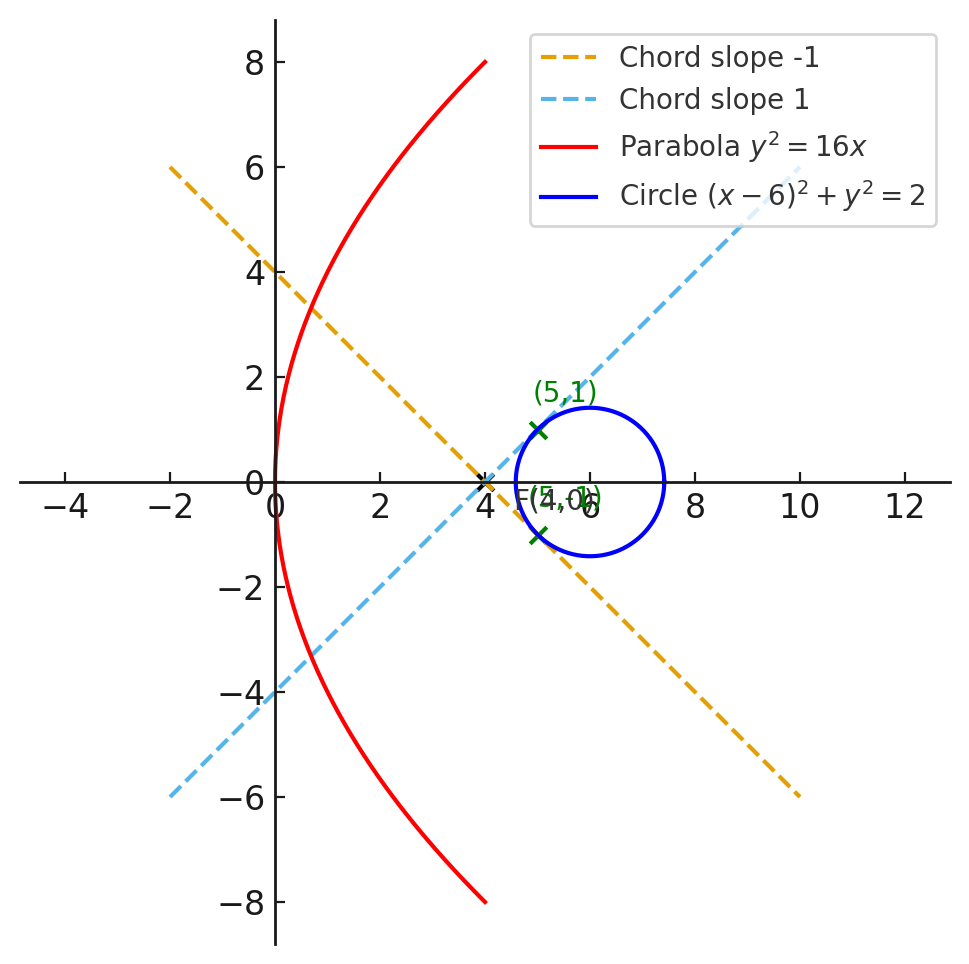
\includegraphics[width=\columnwidth, height=0.8\textheight, keepaspectratio]{figs/tangent.png}     
\end{frame}
\end{document}